 
\section{Paketų atsiskyrimas ir deformacija}
\label{app:video}

\begin{figure}
\subfloat[\(t=0.001\)ms]{\label{video:1}
\centerline{\includegraphics[height=0.28\textheight]{./media/video/00001.png}
}}\\
\subfloat[\(t=0.005\)ms]{\label{video:2}
\centerline{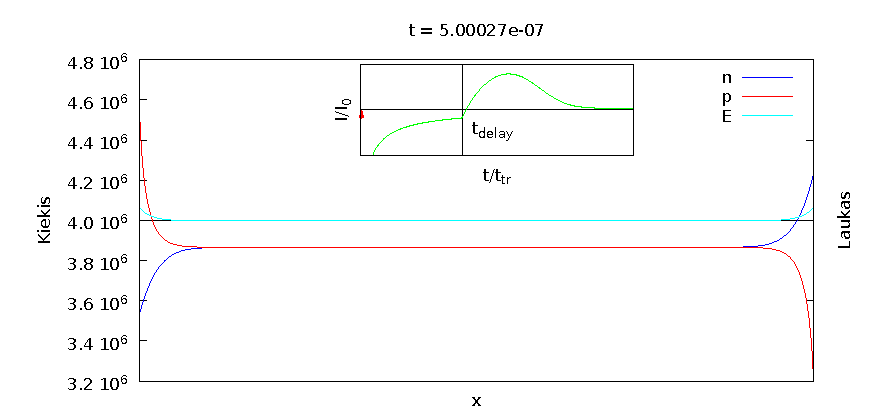
\includegraphics[height=0.28\textheight]{./media/video/00005.png}
}}\\
\subfloat[\(t=0.02\)ms]{\label{video:3}
\centerline{\includegraphics[height=0.28\textheight]{./media/video/00020.png}
}}
\caption{Simuliacijos būsenos kitimas laike}
\end{figure}

\begin{figure}
\ContinuedFloat
\subfloat[\(t=0.08\)ms]{\label{video:4}
\centerline{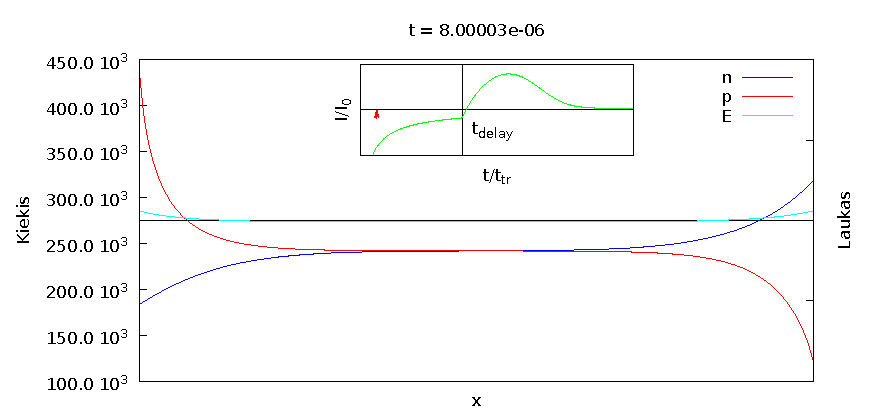
\includegraphics[height=0.28\textheight]{./media/video/00080.png}
}}\\
\subfloat[\(t=0.24\)ms]{\label{video:5}
\centerline{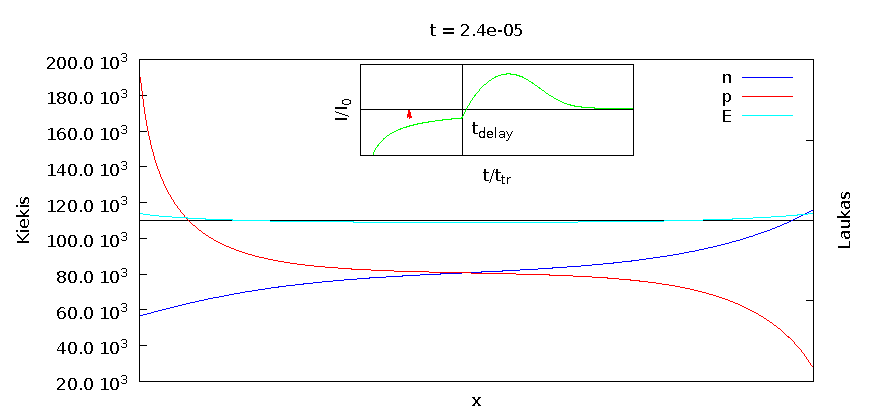
\includegraphics[height=0.28\textheight]{./media/video/00240.png}
}}\\
\subfloat[\(t=0.5\)ms]{\label{video:6}
\centerline{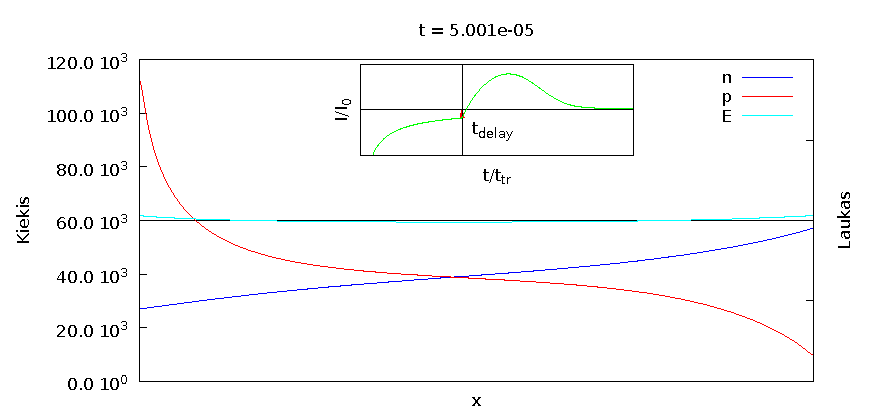
\includegraphics[height=0.28\textheight]{./media/video/00500.png}
}}
\caption{Simuliacijos būsenos kitimas laike (tęs.)}
\end{figure}

\begin{figure}
\ContinuedFloat
\subfloat[\(t=0.65\)ms]{\label{video:7}
\centerline{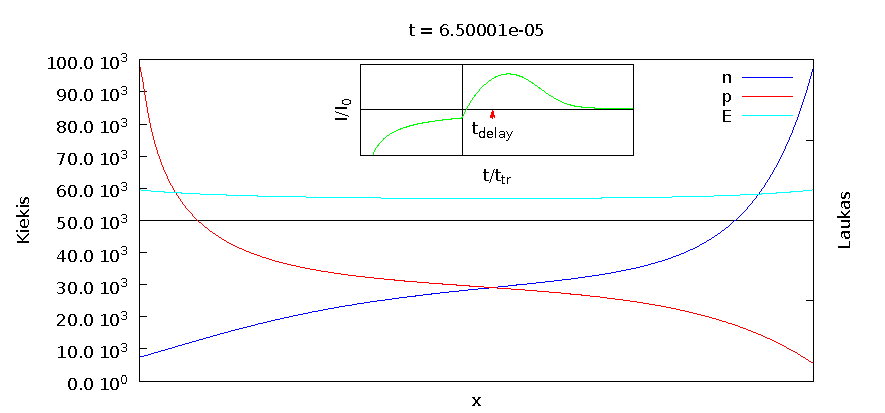
\includegraphics[height=0.28\textheight]{./media/video/00650.png}
}}\\
\subfloat[\(t=0.75\)ms]{\label{video:8}
\centerline{\includegraphics[height=0.28\textheight]{./media/video/00750.png}
}}\\
\subfloat[\(t=0.85\)ms]{\label{video:9}
\centerline{\includegraphics[height=0.28\textheight]{./media/video/00850.png}
}}
\caption{Simuliacijos būsenos kitimas laike (tęs.)}
\label{fig:video}
\end{figure}

Pagal darbe aprašytus simuliacijos parametrus (žr. \ref{page:params} skyrelį) atlikti skaičiavimai, kurių rezultatų pavyzdžiai pateikti \ref{fig:video} pav.
Juose pavaizduoti krūvininkų tankių ir elektrinio lauko pasiskirstymai, skirtingais laiko momentais. Kairėje pusėje pavaizduota apskaičiuotoji CELIV kinetika, čia juoda linija žymi laiko momentą, kurio metu sistemos būsena pavaizduota dešiniajame paveiksliuke. Nekintanti juoda linija žymi CELIV signalo pradžią.
Matome, jog pradiniais laiko momentais (\ref{video:1}, \ref{video:2}, \ref{video:3}, \ref{video:4}) neigiami krūvininkai atsiskiria nuo teigiamų ir plinta į bandinio vidų. Difuzija sukuria srovę nukreiptą gradiento mažėjimo kryptimi ir atskiria paketų masės centrus. Tarp atskirtų paketų atsiranda elektrinis laukas, taigi kartu ir dreifo srovė. Po kurio laiko dreifo srovė kompensuoja difuzijos srovę (\ref{video:5}), bendra srovė tampa lygi nuliui. Pusiausvyra nėra pasiekiama, nes kol krūvininkų paketas dėl difuzijos judėjo tolyn nuo kontakto tol vyko krūvininkų rekombinacija. Dėl rekombinacijos atsiranda neigiamų krūvininkų gradientas nukreiptas priešinga kryptimi (\ref{video:6}). Manoma, kad įtakos šiai srovei turi ir dreifo komponentė, kurios kryptis ir vertė nėra akivaizdi, nes kinta kartu su elektriniu lauku.
Vėliau įjungiamas CELIV įtampos signalas (\ref{video:7}), ir krūvininkai traukiami prie kontaktų (\ref{video:8}, \ref{video:9}).